\documentclass[conference]{sty/ieeeconf}

\usepackage{acro}
\usepackage{siunitx}
\usepackage{url}
\let\labelindent\relax
\usepackage{enumitem}
\usepackage{epsf,graphicx}
\usepackage{epstopdf}
\usepackage{subfigure}
\usepackage{booktabs}

%\acrodef{cap}[CaP]{prostate cancer}
\DeclareAcronym{cap}{
short = CaP,
long = prostate cancer
}
%\acrodef{cade}[CADe]{computer-aided detection}
\DeclareAcronym{cade}{
short = CADe,
long = computer-aided detection
}
%\acrodef{cadx}[CADx]{computer-aided diagnosis}
\DeclareAcronym{cadx}{
short = CADx,
long = computer-aided diagnosis
}
\DeclareAcronym{lm}{
short = LM, 
long = Leung-Malik set
}
%\acrodef{us}[US]{ultrasound}
\DeclareAcronym{us}{
short = UTS,
long = ultrasound
}
%\acrodef{ct}[CT]{computer tomography}
\DeclareAcronym{ct}{
short = CT,
long = computer tomography
}
%\acrodef{cad}[CAD]{computer-aided detection and diagnosis}
\DeclareAcronym{cad}{
short = CAD,
long = computer-aided detection and diagnosis
}
%\acrodef{mri}[MRI]{magnetic resonance imaging}
\DeclareAcronym{mri}{
short = MRI,
long = magnetic resonance imaging
}
%\acrodef{nmr}[NMR]{nuclear magnetic resonance}
\DeclareAcronym{nmr}{
short = NMR,
long = nuclear magnetic resonance
}

\DeclareAcronym{omp}{
  short = OMP,
  long =  orthogonal matching pursuit 
}
\DeclareAcronym{adb}{
  short = AdB, 
  long = AdaBoost
}
\DeclareAcronym{gb}{
  short = GB, 
  long = Gradient Boosting
}

\DeclareAcronym{mp}{
  short = MP,
  long =  Matching Pursuit 
}
%\acrodef{t2w}[T$_2$-W]{T$_2$ Weighted}
\DeclareAcronym{t2w}{
short = T$_2$-W,
long = T$_2$ Weighted
}
%\acrodef{dce}[DCE]{dynamic contrast-enhanced}
\DeclareAcronym{dce}{
short = DCE,
long = dynamic contrast-enhanced
}
%\acrodef{dw}[DW]{diffusion weighted}
\DeclareAcronym{dw}{
short = DW,
long = diffusion weighted
}
%\acrodef{mrsi}[MRSI]{magnetic resonance spectroscopy imaging}
\DeclareAcronym{mrsi}{
short = MRSI,
long = magnetic resonance spectroscopy imaging
}
%\acrodef{bph}[BPH]{benign prostatic hyperplasia}
\DeclareAcronym{bph}{
short = BPH,
long = benign prostatic hyperplasia
}
%\acrodef{pz}[PZ]{peripheral zone}
\DeclareAcronym{pz}{
short = PZ,
long = peripheral zone
}
%\acrodef{cz}[CZ]{central zone}

\DeclareAcronym{mpmri}{
short = mp-MRI,
long = multiparametric \ac{mri}
}
\DeclareAcronym{cz}{
short = CZ,
long = central zone
}
%\acrodef{tz}[TZ]{transitional zone}
\DeclareAcronym{tz}{
short = TZ,
long = transitional zone
}
%\acrodef{cg}[CG]{central gland}
\DeclareAcronym{cg}{
short = CG,
long = central gland
}
%\acrodef{psa}[PSA]{prostate-specific antigen}
\DeclareAcronym{psa}{
short = PSA,
long = prostate-specific antigen
}
%\acrodef{trus}[TRUS]{transrectal ultrasound}
\DeclareAcronym{trus}{
short = TRUS,
long = transrectal ultrasound
}
%\acrodef{tr}[TR]{repetition time}
\DeclareAcronym{tr}{
short = TR,
long = repetition time
}
%\acrodef{te}[TE]{echo time}
\DeclareAcronym{te}{
short = TE,
long = echo time
}
%\acrodef{si}[SI]{signal intensity}
\DeclareAcronym{si}{
short = SI,
long = signal intensity
}
%\acrodef{ees}[EES]{extravascular-extracellular space}
\DeclareAcronym{ees}{
short = EES,
long = extravascular-extracellular space
}
%\acrodef{t1w}[T$_1$-W]{T$_1$ Weighted}
\DeclareAcronym{t1w}{
short = T$_1$-W,
long = T$_1$ Weighted
}
%\acrodef{fse}[FSE]{Fast Spin-Echo}
\DeclareAcronym{fse}{
short = FSE,
long = Fast Spin-Echo
}
%\acrodef{adc}[ADC]{Apparent Diffusion Coeffient}
\DeclareAcronym{adc}{
short = ADC,
long = apparent diffusion coefficient
}
%\acrodef{roi}[ROI]{region of interest}
\DeclareAcronym{roi}{
short = ROI,
long = region of interest
}
%\acrodef{cse}[CSE]{chemical shift effect}
\DeclareAcronym{cse}{
short = CSE,
long = chemical shift effect
}
%\acrodef{snr}[SNR]{signal-to-noise}
\DeclareAcronym{snr}{
short = SNR,
long = signal-to-noise
}
\DeclareAcronym{se}{
short = SE, 
long = sensitivity
}
\DeclareAcronym{sp}{
short = SP, 
long = specificity
}
%\acrodef{gs}[GS]{Gleason score}
\DeclareAcronym{gs}{
short = GS,
long = Gleason score
}
%\acrodef{ersspc}[ERSSPC]{European Randomized Study of Screening for Prostate Cancer}
\DeclareAcronym{ersspc}{
short = ERSSPC,
long = European randomized study of screening for prostate cancer
}
%\acrodef{plco}[PLCO]{Prostate, Lung, Colorectal and Ovarian}
\DeclareAcronym{plco}{
short = PLCO,
long = prostate lung colorectal and ovarian
}
%\acrodef{fig}[Fig.]{figure}
\DeclareAcronym{fig}{
short = Fig.,
long = figure,
class = latex
}
\DeclareAcronym{tab}{
short = Table,
long = table,
class = latex
}
\DeclareAcronym{eq}{
short = Eq.,
long = equation,
class = latex
}
\DeclareAcronym{sec}{
short = Sect.,
long = section,
class = latex
}
\DeclareAcronym{chp}{
short = Chap.,
long = Chapter,
class = latex
}

\DeclareAcronym{fov}{
short = FOV,
long = field of view
}
\DeclareAcronym{dwt}{
short = DWT,
long = discrete wavelet transform
}
\DeclareAcronym{dwst}{
short = DWST,
long = discrete wavelet squared transform
}
\DeclareAcronym{map}{
short = MAP,
long = maximum \textit{a posteriori}
}
\DeclareAcronym{ml}{
short = ML,
long = maximum likelihood
}
\DeclareAcronym{mle}{
short = MLE,
long = maximum likelihood estimation
}
\DeclareAcronym{mrf}{
short = MRF,
long = Markov random field
}
\DeclareAcronym{itk}{
short = ITK,
long = Insight Segmentation and Registration Toolkit
}
\DeclareAcronym{es}{
short = ES,
long = Evolution Strategy
}
\DeclareAcronym{scf}{
short = SCF,
long = sparse coded features
}
\DeclareAcronym{bow}{
short = BoW,
long = bag of words
}
\DeclareAcronym{pdf}{
short = PDF,
long = probability density function
}
\DeclareAcronym{gscale}{
short = \textit{g}-scale,
long = generalized scale
}
\DeclareAcronym{aif}{
short = AIF,
long = arterial input function
}
\DeclareAcronym{svd}{
short = SVD,
long = singular value decomposition
}
\DeclareAcronym{mse}{
short = MSE,
long = mean squared error
}
\DeclareAcronym{mi}{
short = MI,
long = mutual information
}
\DeclareAcronym{mantra}{
short = MANTRA,
long = multi-attribute non-initializing texture reconstruction based active shape model
}
\DeclareAcronym{asm}{
short = ASM,
long = active shape model
}
\DeclareAcronym{pca}{
short = PCA,
long = principal components analysis
}
\DeclareAcronym{weritas}{
short = WERITAS,
long = weighted ensemble of regional image textures for active shape model segmentation
}
\DeclareAcronym{staple}{
short = STAPLE,
long = simultaneous truth and performance level estimation
}
\DeclareAcronym{lda}{
short = LDA,
long = linear discriminant analysis
}
\DeclareAcronym{lbp}{
short = LBP,
long = local binary pattern
}
\DeclareAcronym{tps}{
short = TPS,
long = thin plate spline
}
\DeclareAcronym{acm}{
short = ACM,
long = active contour model
}
\DeclareAcronym{cmi}{
short = CMI,
long = combined mutual information
}
\DeclareAcronym{svm}{
short = SVM,
long = support vector machines
}
\DeclareAcronym{rvm}{
short = RVM,
long = relevant vector machine
}
\DeclareAcronym{rbf}{
short = RBF,
long = radial basis function
}
\DeclareAcronym{knn}{
short = $k$-NN,
long = $k$-nearest neighbour
}
\DeclareAcronym{nn}{
short = NN,
long = neareast neighbour
}
\DeclareAcronym{dct}{
short = DCT,
long = discrete cosine transform
}
\DeclareAcronym{hog}{
short = HOG,
long = histogram of oriented gradient
}
\DeclareAcronym{dft}{
short = DFT,
long = discrete fourier transform
}
\DeclareAcronym{us1}{
short = US,
long = under-sampling
}
\DeclareAcronym{os}{
short = OS,
long = over-sampling
}
\DeclareAcronym{ros}{
short = ROS,
long = random-over-sampling
}
\DeclareAcronym{rus}{
short = RUS,
long = random-under-sampling
}
\DeclareAcronym{nm}{
short = NM,
long = nearmiss
}
\DeclareAcronym{nm3}{
short = NM-3,
long = nearmiss-3
}
\DeclareAcronym{nm2}{
short = NM-2,
long = nearmiss-2
}
\DeclareAcronym{nm1}{
short = NM-1,
long = nearmiss-1
}
\DeclareAcronym{iht}{
short = IHT,
long = instance-hardness-threshold
}
\DeclareAcronym{smote}{
short = SMOTE,
long = synthetic minority over-sampling techniques
}
\DeclareAcronym{smoteb1}{
short = SMOTE-b1,
long = SMOTE-borderline1
}
\DeclareAcronym{smoteb2}{
short = SMOTE-b2,
long = SMOTE-borderline2
}
\DeclareAcronym{mrmr}{
short = mRMR,
long = minimum redundancy maximum relevance
}
\DeclareAcronym{lle}{
short = LLE,
long = locally linear embedding
}
\DeclareAcronym{ica}{
short = ICA,
long = independent components analysis
}
\DeclareAcronym{qda}{
short = QDA,
long = quadratic discriminant analysis
}
\DeclareAcronym{id3}{
short = ID3,
long = iterative dichotomiser 3
}
\DeclareAcronym{cart}{
short = CART,
long = classification and regression tree
}
\DeclareAcronym{bagging}{
short = bagging,
long = bootsrap aggregating
}
\DeclareAcronym{loo}{
short = LOOCV,
long = leave-one-out cross-validation
}
\DeclareAcronym{lopo}{
short = LOPO CV,
long = leave-one-patient-out cross-validation
}

\DeclareAcronym{kcv}{
short = $k$-CV,
long = $k$-fold cross-validation
}
\DeclareAcronym{roc}{
short = ROC,
long = receiver operating characteristic
}
\DeclareAcronym{froc}{
short = FROC,
long = free-response receiver operating characteristic
}
\DeclareAcronym{auc}{
short = AUC,
long = area under the curve
}
\DeclareAcronym{rmse}{
short = RMSD,
long = root-mean-square deviation
}
\DeclareAcronym{rms}{
  short = RMS,
  long = root mean square
}
\DeclareAcronym{srsf}{
  short = SRSF,
  long =  square-root slope function
}
\DeclareAcronym{pun}{
short = PUN,
long = phenomenological universalities
}
\DeclareAcronym{etl}{
short = ETL,
long = echo train ength
}

\DeclareAcronym{rf}{
short = RF,
long = random forest
}
\DeclareAcronym{dna}{
short = DNA,
long = deoxyribonucleic acid
}

\DeclareAcronym{glcm}{
short = GLCM,
long = gray-level co-occurence matrix
}

\DeclareAcronym{iccvb}{
short = I2Cvb,
long = initiative for collaborative computer vision benchmarking
}

\DeclareAcronym{mloss}{
short = MLOSS 2015,
long = machine learning open source software 2015
}

\DeclareAcronym{ci}{
short = CI,
long = continuous integration
}

\DeclareAcronym{cern}{
short = CERN,
long = european organization for nuclear research
}

\DeclareAcronym{doi}{
short = DOI,
long = digital object identifier
}

\DeclareAcronym{pd}{
short = PD,
long = proton density
}

\DeclareAcronym{anova}{
short = ANOVA,
long = analysis of variance
}


\DeclareSIUnit\ppm{ppm}
\DeclareSIUnit\px{px}

% correct bad hyphenation here
\hyphenation{op-tical net-works semi-conduc-tor IEEEtran}


\begin{document}

\title{Computer-Aided Detection for Prostate Cancer Detection based on Multi-Parametric Magnetic Resonance Imaging}

\author{\authorblockN{Guillaume Lema\^{i}tre\authorrefmark{1},
Robert Mart\'i\authorrefmark{2},
Mojdeh Rastgoo\authorrefmark{3} and
Fabrice M\'eriaudeau\authorrefmark{4}\authorrefmark{5}}
\authorblockA{\authorrefmark{1} Parietal team, Inria, CEA, Universit\'e Paris-Saclay, 1 Rue Honor\'e d'Estienne d'Orves, 91120 Palaiseau}
\authorblockA{\authorrefmark{2} ViCOROB, Universitat de Girona, Campus Montilivi, Edifici P4, 17071 Girona}
\authorblockA{\authorrefmark{3} LE2I UMR6306, CNRS, Arts et M\'etiers, Univ. Bourgogne Franche-Comt\'e, 12 rue de la Fonderie, 71200 Le Creusot}
\authorblockA{\authorrefmark{4} CISIR, Electrical \& Electronic Engineering Department,Universiti Teknologi Petronas, 32610 Seri Iskandar, Perak}
\authorblockA{\authorrefmark{5} Corresponding author: fabrice.meriaudeau@utp.edu.my}}

\maketitle

\begin{abstract}
\Ac{cap} is the second most diagnosed cancer in men all over the world.
In the last decades, new imaging techniques based on \ac{mri} have been developed improving diagnosis.
In practice, diagnosis is affected by multiple factors such as observer variability and visibility and complexity of the lesions.
In this regard, \ac{cad} systems are being designed to help radiologists in their clinical practice.
We propose a \ac{cad} system taking advantage of all MRI modalities (i.e.,
\acs*{t2w}-\acs*{mri}, \acs*{dce}-\acs*{mri}, \ac{dw}-\acs*{mri}, \acs*{mrsi}).
The aim of this \ac{cad} system was to provide a probabilistic map of cancer
location in the prostate.
We extensively tested our proposed \ac{cad} using different fusion approaches
to combine the features provided by each modality.
The source code and the dataset have been released.
\end{abstract}

\acresetall

\section{Introduction}
Current \ac{cap} screening consists of 3 different stages.
First, \ac{psa} control is performed to distinguish between low- and
high-risk \ac{cap}.
To assert such diagnosis, samples are taken during prostate biopsy and
analyzed to make an accurate prognosis of the \ac{cap}.

Although \ac{psa} screening has been shown to improve early detection
of \ac{cap}~\cite{Chou2011}, its lack of reliability motivates further
investigations using \ac{mri}-based \ac{cad}.
Consequently, current research is focused on identifying new
biological markers to replace \ac{psa}-based
screening~\cite{Brenner2013}.
Until such research comes to fruition, these needs can be met through
active-surveillance strategy using \ac{mpmri}
techniques~\cite{Moore2013}.

Lemaitre\,\emph{et~al.} recently reviewed
more than 50 research works that focused on \ac{cad} system for
\ac{cap}~\cite{Lemaitre2015}.
These studies are based on \ac{cad} systems that consists of the
following steps:
(i) pre-processing,
(ii) segmentation,
(iii) registration,
(iv) feature detection,
(v) feature selection-extraction, and
(vi) finally classification.

The reviewed \ac{mpmri}-based \ac{cad} used 2 to 3
\ac{mri} modalities among \ac{t2w}-\ac{mri}, \ac{dce}-\ac{mri}, and
\ac{dw}-\ac{mri}, discarding the potential discriminative power of
\ac{mrsi}.
Furthermore, only half of these studies tackled the challenging
detection of \ac{cap} in the \ac{cg}.
Additionally, none of the works investigated the issue related to
feature balancing when developing their \ac{cad} systems.
Finally, none of the datasets nor source codes used have been
released, making impossible the possibilities to compare the methods.

In this work, we propose a \ac{cad} system to detect \ac{cap} in
\ac{pz} and \ac{cg}, using the 4 aformentioned \ac{mri}
modalities.
The ultimate goal of the current \ac{cad} system is to provide a probabilistic
map of the cancer within the prostate.
Therefore, each voxel in the prostate will be classified as healthy or
cancerous.
The dataset used and the source code developed are released for future
comparisons and reproducibility.

\section{Methodology}\label{sec:chp6:method}

\subsection{Materials}

The \ac{mpmri} data are acquired from a cohort of patients with
higher-than-normal level of \ac{psa}.
Acquisition is achieved with a \SI{3}{\tesla} whole body
\ac{mri} scanner (Siemens Magnetom Trio TIM, Erlangen, Germany) using
sequences to obtain \ac{t2w}-\ac{mri}, \ac{dce}-\ac{mri},
\ac{dw}-\ac{mri}, and \ac{mrsi}.
In addition of the \ac{mri} examination, these patients also have undergone
a \ac{trus} guided-biopsy.
The dataset is composed of 17 of which have biopsies that were positive for
\ac{cap}.
In all 12 patients have a \ac{cap} in the \ac{pz}, 3 patients
have \ac{cap} in the \ac{cg}, 2 patients have invasive \ac{cap} in
both the \ac{pz} and the \ac{cg}.
An experienced radiologist segmented the prostate organ --- on
\ac{t2w}-\ac{mri}, \ac{dce}-\ac{mri}, and \ac{adc} --- as
well as the prostate zones --- i.e., \ac{pz} and \ac{cg} ---, and
\ac{cap} on the \ac{t2w}-\ac{mri}.
The full description and the data set are available at \acs*{iccvb}
website\footnote{\url{http://i2cvb.github.io/}}~\cite{Lemaitre2016thesis}.

\subsection{\acs*{cad} pipeline for \acs*{cap}}

Our \ac{mpmri} \ac{cad} system consists of 7 different steps:
pre-processing, segmentation, registration, feature detection, feature
balancing, feature selection/extraction, and finally classification.
The different source codes are publicly
available\footnote{\url{https://github.com/I2Cvb/mp-mri-prostate}}.

\subsubsection{Pre-processing}\label{subsec:chp6:method:PP}

Normalization is, a crucial step to reduce the inter-patient
variations which allows to improve the learning during the
classification stage.
However, the \ac{mri} modalities provide specific type of data --- static
\emph{vs.} dynamic information, images \emph{vs.} signals --- that
required a dedicated pre-processing.
Therefore, we pre-process differently the data:
\ac{t2w}-\ac{mri} is normalized using a Rician
a-priori that has been shown to be better than the traditional
$z$-score~\cite{lemaitre2016normalization}.
In contrast to \ac{t2w}-\ac{mri}, in \ac{adc} map the \ac{pdf} within the
prostate does not follow a known distribution and thus one cannot use
a parametric model to normalize these images and a non-parametric
piecewise-linear normalization~\cite{Nyul2000} is the best option for
this case.
\ac{dce}-\ac{mri} is a dynamic sequence and the data are normalized
based on a mean kinetic expression registration as proposed
in~\cite{Lemaitre2016thesis}.
Finally, the \ac{mrsi} modality has been pre-processed to correct the
phase, suppress the baseline, and align the frequencies~\cite{Parfait2012}.

\subsubsection{Segmentation and registration}\label{subsec:chp6:method:Seg-Reg}

For this work, our radiologist has manually segmented the prostate
organs on the different modalities.
However, the segmented prostate needs to be registered before to
extract features.
Therefore, the patients motion during the \ac{dce}-\ac{mri} is corrected using
a rigid registration with an \ac{mse} similarity metric and a gradient descent
optimizer.
Subsequently, the \ac{t2w}-\ac{mri} and \ac{dce}-\ac{mri} are co-registered
using a rigid transformation and the delineation of the prostate gland, using
the same metric and optimizer previously mentioned.
\ac{adc} maps and \ac{t2w}-\ac{mri} are also co-registered with the same
strategy.
Additionally, volumes from all modalities have been interpolated to the
resolution of \ac{t2w}-\ac{mri}.

\subsubsection{Feature detection}\label{subsec:chp6:method:fea-det}
Similarly to the pre-processing, specific features are extracted
depending of the specificity of each \ac{mri} modality.
\begin{description}
\item[\ac{t2w}-\ac{mri} and \ac{adc} map features]
Additionally to the normalized intensity, edge- and texture-based
features are commonly extracted from \ac{t2w}-\ac{mri} and \ac{adc}
map.
The following set of filters characterizing edges have been used: (i)
Kirsch, (ii) Laplacian, (iii) Prewitt, (iv) Scharr, (v) Sobel, and
(vi) Gabor.
Except for the Kirsch filter, the other filters are applied in 3D,
taking advantage of the volume information instead of slice
information, as it is usually done.
Additionally, features based on phase congruency are
computed~\cite{kovesi1999image}.
To characterize the local texture, both second-order \ac{glcm}-based
features~\cite{Haralick1973} and rotation invariant and uniform
\ac{lbp}~\cite{ojala2002multiresolution} are extracted.
To encode 3D information, the 13 first Haralick features are computed
for the 13 possible directions.
For the same reason, the \ac{lbp} codes are computed for the
three-orthogonal-planes of each \ac{mri} volume.
All these features are extracted at each voxel of the volume.

\item[\ac{dce}-\ac{mri} features]
In brief, the entire enhanced signal, semi-quantitative~\cite{Huisman2001}, and
quantitative-based
models~\cite{brix1991pharmacokinetic,hoffmann1995pharmacokinetic,tofts1995quantitative,giannini2015fully}
are computed.

\item[\ac{mrsi} features]
Three different techniques are used to extract
discriminative features: (i) relative quantification based on
metabolite quantification, (ii) relative
quantification based on bounds integration, and (iii) spectra
extraction from \SIrange{2}{4}{\ppm}~\cite{Lemaitre2016thesis}.

\item[Anatomical features]
Four different metrics are computed based on the relative distance to the
prostate boundary as well as the prostate center, and the relative
position in the Euclidean and cylindrical coordinate
systems~\cite{Chen2002,Litjens2014}.

\end{description}

\subsubsection{Feature balancing}\label{subsec:chp6:method:fea-bal}
Imbalanced dataset is a common problem in medical imaging.
The number of cancerous voxels is much lower than the number of
``healthy'' voxels for a patient.
This problem compromises the learning process.
Solving the problem of imbalanced is equivalent to under- or
over-sampling part of the dataset to obtain equal number of samples
in both classes.
In this regard, the imbalanced dataset was under-sampled using the different
variant of \ac{nm}~\cite{mani2003knn} and the \ac{iht}~\cite{smith2014instance}
algorithm.
In addition, the dataset was also balanced using over-sampling methods, namely
different variant of \ac{smote}~\cite{chawla2002smote,han2005borderline}.
Those algorithms were developed and made publicly available in the
\texttt{scikit-learn-contrib
  imbalanced-learn}\footnote{\url{http://contrib.scikit-learn.org/imbalanced-learn/}}
python package~\cite{imblearn}.

\subsubsection{Feature selection and extraction}\label{subsec:chp6:method:fea-sel}

Feature selection and extraction are used in our experiment.
\ac{mrsi} and \ac{dce}-\ac{mri} are decomposed using three feature
extraction methods: \ac{pca}, sparse-\ac{pca}, and \ac{ica} are used
to decompose signal-based data.
Additionally to feature extraction, two methods of feature selection
are used: (i) the one-way \ac{anova} and (ii) the Gini importance
obtained while learning the \ac{rf} classifiers.
The \texttt{scikit-learn}\footnote{\url{http://scikit-learn.org/stable/}}
python package provides all those methods and was use in our
experiment~\cite{pedregosa2011scikit}.

\subsubsection{Classification}\label{subsec:chp6:method:clas}

\ac{rf} has been chosen as our base classifier to perform classification of
individual modality as well as the combination of modalities.
\ac{rf} and more generally decision trees do not required to scale features and
provide a feature selection add-on by analyzing the feature importance derived
from the impurity improvement successive splits.
Additionally, we use stacking to create ensemble of base learners using a
meta-classifier~\cite{wolpert1992stacked}, namely \ac{adb} and \ac{gb}.

\section{Results and evaluation} \label{sc:results}

\begin{table*}
  \caption{Selected feature and number of occurrence for \acs*{t2w}-\acs*{mri}, \acs*{adc} map, and one all the features are concatenated.}
  \centering
  \begin{tabular}{llllll}
    \toprule
    \multicolumn{1}{c}{\textbf{\acs*{t2w}-\acs*{mri}}} & \multicolumn{1}{c}{\textbf{\acs*{adc}}} & \multicolumn{1}{c}{\textbf{\acs*{t2w}-\acs*{mri}}} & \multicolumn{1}{c}{\textbf{\acs*{adc}}} & \multicolumn{1}{c}{\textbf{\acs*{dce}-\acs*{mri}}} & \multicolumn{1}{c}{\textbf{\acs*{mrsi}}} \\
    \cmidrule(lr){1-1} \cmidrule(lr){2-2} \cmidrule(lr){3-6}
    8 edges & 1 \acs*{dct} & 113 Gabor filters & 53 Gabor filters & 14 samples  & 78 samples \\
    155 Gabor filters & 32 Gabor filters & 1 phase congruency & 2 phase congruency & & \\
    2 Haralick features & 1 phase congruency & 4 edges & & & \\
    1 intensity & & 1 intensity & & & \\
    4 \acs*{lbp} & & & & & \\
    2 phase congruency & & & & & \\
    \cmidrule(lr){1-1} \cmidrule(lr){2-2} \cmidrule(lr){3-6}
    \multicolumn{1}{c}{\textbf{172 features}} & \multicolumn{1}{c}{\textbf{34 features}} & \multicolumn{4}{c}{\textbf{267 features}} \\
    \bottomrule
  \end{tabular}
  \label{tab:selfeatocc}
\end{table*}

\begin{figure}
\centering
 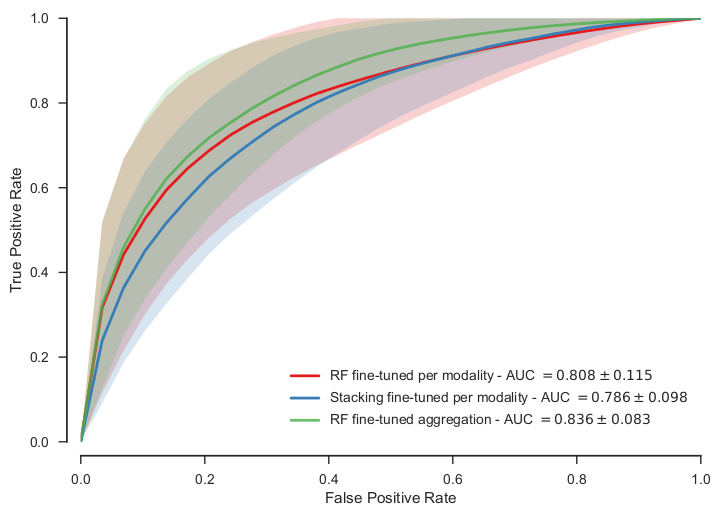
\includegraphics[width=0.9\linewidth]{figures/combine_all.png}
  \caption[Analysis of feature combination approaches after fine
  tuning.]{Analysis of feature combination approaches after fine
    tuning through balancing and feature selection/extraction.}
  \label{fig:res-Ex4}
\end{figure}

Various experiments were run in order to optimize the balancing and
the feature selection strategies~\cite{Lemaitre2016thesis}.
We found that once all features are concatenated together,
\ac{nm3}~\cite{mani2003knn} is the method providing the best
enhancement of the classification performance with an \ac{auc} of $0.824 \pm
0.076$.
Therefore, with this optimal balancing, were here report the
final step consisting of three strategies:
(i) the selected features from each modality (i.e., 331 features) are
concatenated together and used in a \ac{rf} classifier,
(ii) the selected features from each modality (i.e., 331 features) are
used to train a stacking classifier with a \ac{gb} as meta-classifier, and
(iii) the selected features from the concatenated set of feature
(i.e., 267 features) are used to train a single \ac{rf} classifier.

The selected features are presented in Table~\ref{tab:selfeatocc} which
highlights some interesting facts regarding the most efficient features.
On the one hand, the Gabor filters and the phase congruency are always
selected, independently of the strategy and modality during the feature
selection process.
Additionally, edge filters --- i.e., Kirsch, Prewitt, Scharr, and Sobel ---
have been only selected for the \ac{t2w}-\ac{mri}.
A possible explanation might be due to the fact that \ac{t2w}-\ac{mri} is the
modality with the highest spatial resolution and in which the level of details
is the most important.
Subsequently, the intensity feature of the \ac{t2w}-\ac{mri} modality is always
selected, implying that our normalization method proposed
in~\cite{lemaitre2016normalization} is efficient.


\begin{figure}
  \hspace*{\fill}
  \subfigure[\acs*{auc} =
  0.922]{\label{fig:pat634}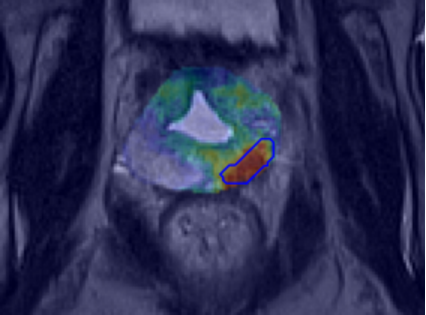
\includegraphics[width=.45\linewidth]{figures/patient_634_foc.pdf}}
 \hfill
 \subfigure[\acs*{auc} =
 0.914]{\label{fig:pat1036}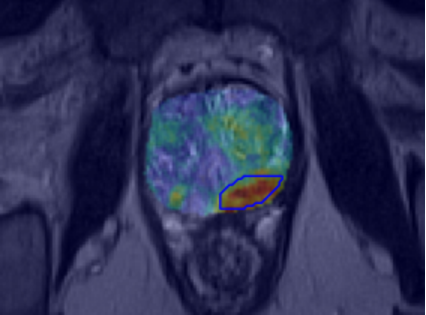
\includegraphics[width=.45\linewidth]{figures/patient_1036_foc.pdf}}
 \hspace*{\fill}
  \caption[Illustration the resulting detection of our \acs*{mpmri}
  \acs*{cad} for \acs*{cap} detection.]{Illustration the resulting
    detection of our \acs*{mpmri} \acs*{cad} for \acs*{cap}
    detection. The blue contours corresponds to the \ac{cap} while the
    jet overlay represents the probability.}
  \label{fig:resultcad}
\end{figure}

The experiments were performed in a \ac{lopo} fashion and a \ac{roc}
analysis is carried out.
The comparative results are shown in \acs{fig}\,\ref{fig:res-Ex4}.
In overall, classification using the fine-tuned features improve the
classification performance.
The third classification configuration is, however, the one which
outperforms others with an \ac{auc} of $0.836 \pm 0.083$.
The improvement in terms of \ac{auc} is of $0.028$ and $0.050$
compared with the 1\textsuperscript{st} and 2\textsuperscript{nd}
configurations, respectively.

In clinical setting, the \ac{auc} score is categorized in 3 levels:
(i) ``acceptable'' discrimination for an \ac{auc} ranging from $0.7$
to $0.8$, (ii) ``excellent'' discrimination for an \ac{auc} ranging
from $0.8$ to $0.9$, and ``outstanding'' discrimination when the
\ac{auc} is over $0.9$~\cite{hosmer2004applied}.
Therefore, the combination of all \ac{mri} modalities in conjunction
with fine-tuning allow to upgrade our \ac{cad} system from an
``acceptable'' to an ``excellent'' discrimination level.

To illustrate qualitatively the results of our \ac{mpmri} \ac{cad}
system, 2 diverse examples are presented in
\acs{fig}\,\ref{fig:resultcad} by overlapping the probability map of
having a \ac{cap} with the original \ac{t2w}-\ac{mri} slice.

\section{Conclusion}

In this paper, we presented one of the the first \ac{cad} system using all
the \ac{mpmri} modalities for prostate cancer detection.
Indeed, \ac{mrsi} has nearly never been used together with the other
modalities.
With an extensive validation approach to select the best
features, the best balancing strategy as well as the best classifier,
we obtained results on a rather complicated dataset of 17 patients
with an average \ac{auc} of $0.836 \pm 0.083$ which put our system in the
state-of-the-art, even so different \ac{cad}s were tested on different
datasets.

As avenues for future research, one could switch from voxel-based
classification to super-voxel classification such that spatial structure are
classified instead of voxel.
In addition, the registration relies on the segmentation of the prostate gland
which was provided by our doctors.
To be used in a clinical environment, this step need to be fully automatized.

\bibliographystyle{sty/IEEEtran}
\IEEEtriggeratref{13}
\bibliography{IEEEabrv,bibliography}

\end{document}
